% YZM5110 Research Project report -- DRAFT
% Build:  python scripts/make_report_tables.py && (cd report && tectonic main.tex)
% Every number below is either a macro from generated/numbers.tex (measured, from results/),
% a table from generated/tab_*.tex, or a published value cited to its source.
\documentclass[11pt,a4paper]{article}
\usepackage[margin=2.3cm]{geometry}
\usepackage[T1]{fontenc}
\usepackage{lmodern}
\usepackage{microtype}
\usepackage{amsmath,amssymb}
\usepackage{booktabs,array,longtable,tabularx}
\usepackage{pdflscape}
\usepackage{graphicx}
\usepackage{adjustbox}
\usepackage[section]{placeins}
\usepackage{xcolor}
\usepackage{enumitem}
\usepackage[hidelinks]{hyperref}
\usepackage{caption}
\captionsetup{font=small,labelfont=bf}
\setlist{itemsep=2pt,topsep=3pt}
\emergencystretch=3em
\usepackage{fvextra}
\graphicspath{{../results/figures/}}
% generated by scripts/make_report_tables.py -- do not edit
\newcommand{\nQueries}{451}
\newcommand{\nPages}{500}
\newcommand{\nDup}{22}
\newcommand{\pubCard}{0.585}
\newcommand{\pubPaper}{0.544}
\newcommand{\fullB}{0.575}
\newcommand{\fullA}{0.391}
\newcommand{\fullBGE}{0.249}
\newcommand{\gapCardPts}{$-$0.94}
\newcommand{\pubBMtwentyfive}{0.368}
\newcommand{\pubBGE}{0.257}
\newcommand{\fullBnodup}{0.601}
\newcommand{\nDev}{226}
\newcommand{\devB}{0.580}
\newcommand{\devA}{0.400}
\newcommand{\devBGE}{0.235}
\newcommand{\devCkone}{0.534}
\newcommand{\devDkone}{0.526}
\newcommand{\devCksixty}{0.467}
\newcommand{\devDksixty}{0.422}
\newcommand{\devCw}{0.585}
\newcommand{\devDw}{0.580}
\newcommand{\devCwGainPts}{+0.47}
\newcommand{\nWgrid}{9}
\newcommand{\nKgrid}{10}
\newcommand{\nTest}{225}
\newcommand{\testA}{0.382}
\newcommand{\testACI}{[0.323, 0.441]}
\newcommand{\deltaA}{$-$0.188}
\newcommand{\deltaACI}{[$-$0.237, $-$0.142]}
\newcommand{\pHolmA}{$<$0.001}
\newcommand{\pA}{$<$0.001}
\newcommand{\wtlA}{10/144/71}
\newcommand{\testBGE}{0.262}
\newcommand{\testBGECI}{[0.209, 0.317]}
\newcommand{\deltaBGE}{$-$0.308}
\newcommand{\deltaBGECI}{[$-$0.364, $-$0.252]}
\newcommand{\pHolmBGE}{$<$0.001}
\newcommand{\pBGE}{$<$0.001}
\newcommand{\wtlBGE}{5/122/98}
\newcommand{\testB}{0.570}
\newcommand{\testBCI}{[0.510, 0.627]}
\newcommand{\testC}{0.516}
\newcommand{\testCCI}{[0.457, 0.574]}
\newcommand{\deltaC}{$-$0.054}
\newcommand{\deltaCCI}{[$-$0.076, $-$0.032]}
\newcommand{\pHolmC}{$<$0.001}
\newcommand{\pC}{$<$0.001}
\newcommand{\wtlC}{9/167/49}
\newcommand{\testD}{0.519}
\newcommand{\testDCI}{[0.460, 0.578]}
\newcommand{\deltaD}{$-$0.051}
\newcommand{\deltaDCI}{[$-$0.072, $-$0.030]}
\newcommand{\pHolmD}{$<$0.001}
\newcommand{\pD}{$<$0.001}
\newcommand{\wtlD}{4/171/50}
\newcommand{\testCw}{0.571}
\newcommand{\testCwCI}{[0.511, 0.629]}
\newcommand{\deltaCw}{+0.001}
\newcommand{\deltaCwCI}{[$-$0.002, +0.005]}
\newcommand{\pHolmCw}{1.000}
\newcommand{\pCw}{0.937}
\newcommand{\wtlCw}{2/220/3}
\newcommand{\testDw}{0.570}
\newcommand{\testDwCI}{[0.510, 0.627]}
\newcommand{\deltaDw}{+0.000}
\newcommand{\deltaDwCI}{[+0.000, +0.000]}
\newcommand{\pHolmDw}{1.000}
\newcommand{\pDw}{1.000}
\newcommand{\wtlDw}{0/225/0}
\newcommand{\deltaCvsD}{$-$0.003}
\newcommand{\deltaCvsDCI}{[$-$0.027, +0.021]}
\newcommand{\pCvsD}{0.844}
\newcommand{\wtlCvsD}{25/174/26}
\newcommand{\pCwvsDw}{0.937}
\newcommand{\nexact}{93}
\newcommand{\typeexactA}{0.617}
\newcommand{\typeexactB}{0.833}
\newcommand{\typeexactC}{0.774}
\newcommand{\typeexactD}{0.771}
\newcommand{\ngeneral}{115}
\newcommand{\typegeneralA}{0.231}
\newcommand{\typegeneralB}{0.391}
\newcommand{\typegeneralC}{0.345}
\newcommand{\typegeneralD}{0.343}
\newcommand{\nvisual}{17}
\newcommand{\typevisualA}{0.118}
\newcommand{\typevisualB}{0.339}
\newcommand{\typevisualC}{0.265}
\newcommand{\typevisualD}{0.331}
\newcommand{\nNoDup}{212}
\newcommand{\noDupB}{0.598}
\newcommand{\noDupC}{0.542}
\newcommand{\noDupDeltaC}{$-$0.056}
\newcommand{\noDupDeltaCw}{+0.001}
\newcommand{\peakGPU}{15.8}
\newcommand{\latB}{51.3}
\newcommand{\latA}{0.12}
\newcommand{\latBGE}{29.0}
\newcommand{\fusionOverhead}{0.13}
\newcommand{\idxB}{111.7}
\newcommand{\sizeB}{126}
\newcommand{\headallAnotB}{3}
\newcommand{\headallBnotA}{50}
\newcommand{\headexactAnotB}{0}
\newcommand{\headexactBnotA}{22}
\newcommand{\headgeneralAnotB}{3}
\newcommand{\headgeneralBnotA}{23}
\newcommand{\headvisualAnotB}{0}
\newcommand{\headvisualBnotA}{5}
\newcommand{\hitB}{147}
\newcommand{\hitA}{100}
\newcommand{\oracle}{150}
\newcommand{\bothMiss}{75}
\newcommand{\oracleNDCG}{0.588}
\newcommand{\oracleGainPts}{+1.8}
\newcommand{\oracleAbetter}{10}
\newcommand{\cWins}{9}
\newcommand{\cLosses}{49}
\newcommand{\cLossBMmissed}{42}
\newcommand{\cwChanged}{5}
\newcommand{\ovAhit}{0.73}
\newcommand{\ovAmiss}{0.18}
\newcommand{\ovZeroN}{75}
\newcommand{\ovZeroA}{0}
\newcommand{\ovZeroB}{23}
\newcommand{\ovOneN}{43}
\newcommand{\ovOneA}{91}
\newcommand{\ovOneB}{95}


% ---- claim-type labels (assignment: keep published / interpretation / measured apart) -------------
\definecolor{tagP}{HTML}{2a78d6}\definecolor{tagI}{HTML}{8a6d00}\definecolor{tagM}{HTML}{1b7a55}\definecolor{tagH}{HTML}{9b3d8a}
\newcommand{\lbl}[2]{\textsf{\scriptsize\textcolor{#1}{[#2]}}}
\newcommand{\Pub}{\lbl{tagP}{Published}}
\newcommand{\Int}{\lbl{tagI}{Interpretation}}
\newcommand{\Mea}{\lbl{tagM}{Measured}}
\newcommand{\Hyp}{\lbl{tagH}{Hypothesis}}
\newcommand{\todo}[1]{\textcolor{red}{\textbf{[TODO: #1]}}}
\newcommand{\repo}{\url{https://github.com/ismailucrn/colpali-hybrid-retrieval}}
\newcommand{\file}[1]{\texttt{\small\hyphenchar\font=`\/ #1}}

\title{Does a Lexical Signal Still Help a Visual Retriever?\\[2pt]
\large Reproducing ColPali on ViDoRe DocVQA and Testing BM25 Fusion}
\author{\todo{First name LAST NAME} \quad (\todo{student ID})\\
YZM5110 Multimodal Learning --- Research Project}
\date{Draft, \today}

\begin{document}
\maketitle
\begin{center}
\fbox{\parbox{0.9\linewidth}{\centering
\textbf{Repository:} \repo\\
Submitted version: tag \texttt{v1.0-submission} \todo{create the tag and put its commit hash here}}}
\end{center}

\begin{abstract}
\noindent ColPali retrieves document pages directly from their images with a vision--language model and late interaction, replacing the OCR-and-chunking pipeline. Text retrieval has long benefited from fusing lexical (BM25) and dense rankings, so we ask whether a lexical signal still adds anything once retrieval works on page images, and for which queries.
We reproduce ColPali (checkpoint v1.3) on ViDoRe DocVQA: nDCG@5 \fullB{} measured vs \pubCard{} reported by the authors (\gapCardPts{} points, inside a tolerance fixed before the run).
We then test reciprocal rank fusion (RRF) of ColPali with BM25 over the benchmark's OCR text, against a control that fuses ColPali with a dense text retriever (BGE-M3) instead. Fusion settings are chosen on a development split, and the test split is used once.
The result is negative. Equal-weight RRF lowers test nDCG@5 from \testB{} to \testC{} ($\Delta$ \deltaC{}, 95\% CI \deltaCCI{}, Holm-corrected $p$ \pHolmC{}), and the dense control behaves the same ($\Delta$ C$-$D \deltaCvsD{}, $p$ = \pCvsD{}). A dev-tuned weighted RRF only matches ColPali (\deltaCw{}, $p$ = \pCw{}).
Failure analysis explains why. BM25 finds the gold page that ColPali misses on only \headallAnotB{} of \nTest{} test queries, and ColPali is already strongest on the exact-match queries where we expected BM25 to help. BM25 succeeds only when the query's words survive OCR, so fusion mostly imports its errors.
\end{abstract}

\paragraph{How to read this report.} The assignment asks to keep four kinds of statements apart. We label them where it matters: \Pub{} = reported by the cited authors; \Mea{} = obtained by us (every such number is generated from a committed file in \file{results/} by \file{scripts/make\_report\_tables.py}); \Int{} = our reading of a paper or result; \Hyp{} = expected but not tested.

% =====================================================================================================
\section{Research question, scope, motivation and contributions}
\label{sec:rq}

\paragraph{Motivation.}
Retrieval-augmented systems over PDFs usually first turn each page into text (layout detection, OCR, chunking) and then embed the text. ColPali~\cite{colpali} skips that step: it embeds the page \emph{image} with a vision--language model and scores it against the text query by late interaction. \Pub{} It beats every text pipeline on the ViDoRe benchmark, including BM25 and BGE-M3 over OCR text~\cite[Table~2]{colpali}.
In text retrieval, however, a cheap and widely used improvement is to \emph{fuse} a lexical ranking (BM25) with a dense one, because the two fail on different queries~\cite{bruch,cormack}. \Int{} Dense and visual retrievers are often said to struggle with exact strings such as numbers, codes and names, which are exactly what BM25 matches. If that holds for ColPali, a BM25 signal should still help, at almost no cost.

\paragraph{Research question.}
\emph{Does fusing lexical retrieval (BM25 over page text) with ColPali improve page retrieval over ColPali alone, and for which query types?}
We also ask whether any gain comes from the \emph{lexical} signal specifically, or simply from ensembling ColPali with any second retriever.

\paragraph{Scope.}
Deliberately narrow:
\begin{itemize}
  \item one ViDoRe~v1 task (DocVQA: \nPages{} pages, \nQueries{} queries);
  \item the authors' published checkpoint, inference only, with no training or fine-tuning;
  \item page retrieval only, with no answer generation;
  \item rank-level fusion only (RRF and a weighted variant).
\end{itemize}

\paragraph{Contributions.}
\begin{enumerate}
  \item A traceable reproduction of ColPali v1.3 on DocVQA with the official evaluation protocol. The metric code is checked against MTEB, every run (including failed ones) is logged, and outputs are saved (Section~\ref{sec:repro}).
  \item A pre-registered, controlled test of BM25 + ColPali fusion. It has a dense-text control, a frozen dev/test split, frozen query-type tags, paired significance tests with multiple-comparison correction, and resource measurements (Sections~\ref{sec:improve}--\ref{sec:results}).
  \item A negative result with a mechanism. The failure analysis shows the lexical signal has almost no headroom on this task, and why: lexical overlap after OCR (Section~\ref{sec:failure}).
  \item A literature matrix of eight papers. It shows that text + visual fusion has been tried only recently, with mixed and uncontrolled results (Section~\ref{sec:lit}).
\end{enumerate}

% =====================================================================================================
\section{Literature search and critical synthesis}
\label{sec:lit}

\subsection{Search approach}
\begin{enumerate}
  \item \textbf{Seed set.} We started from the main paper (ColPali~\cite{colpali}) and its direct lineage: the paper that introduced late interaction (ColBERT~\cite{colbert}), the benchmark and its successor (ViDoRe~v1 inside~\cite{colpali}; ViDoRe~V2~\cite{vidorev2}), and the closest competing visual retriever (DSE~\cite{dse}).
  \item \textbf{Fusion and text-IR evidence.} We added the method used in our improvement (RRF~\cite{cormack}) and the most detailed analysis of fusion functions for lexical + dense retrieval~\cite{bruch}.
  \item \textbf{Targeted search for the closest prior work.} On 6~Nov 2026 we searched arXiv and the web for work fusing OCR text with ColPali-type retrievers (two queries, listed in \file{docs/literature\_matrix.md}). This found IRPAPERS~\cite{irpapers}, a slide-retrieval study~\cite{slides} and an OCR-versus-vision comparison~\cite{lostocr}.
\end{enumerate}

\noindent\textbf{Inclusion criteria.} A paper was kept if it introduces the reproduced method or a component of it, defines our protocol, is a competing approach, supplies the fusion method or the evidence behind our hypothesis, or directly tests text + visual fusion.
BEIR~\cite{beir}, VisRAG~\cite{visrag} and~\cite{lostocr} are kept as related work only. BEIR does not evaluate fusion, VisRAG is about generation, and \cite{lostocr} has no fusion.

\noindent\textbf{Known bias.} The search was small: two English queries and no citation tracking. Newer or non-arXiv work may be missing.

\noindent\textbf{How details were checked.} Paper details were extracted from the arXiv HTML/PDF versions with AI assistance (Appendix~\ref{app:ai}). Every cell names its section or table in \file{docs/literature\_matrix.md} so that it can be checked against the paper. \todo{author: confirm every cell against the papers}

\subsection{Comparison matrix}
Table~\ref{tab:matrix} condenses the matrix. The full version, with the location of every claim and the open verification items, is in \file{docs/literature\_matrix.md}. All cells are \Pub{} unless marked \Int{}.

\begin{landscape}
\footnotesize
\setlength{\tabcolsep}{3pt}
\renewcommand{\arraystretch}{1.15}
\begin{longtable}{>{\raggedright\arraybackslash}p{2.1cm}>{\raggedright\arraybackslash}p{2.9cm}>{\raggedright\arraybackslash}p{2.4cm}>{\raggedright\arraybackslash}p{3.1cm}>{\raggedright\arraybackslash}p{2.9cm}>{\raggedright\arraybackslash}p{3.3cm}>{\raggedright\arraybackslash}p{2.6cm}>{\raggedright\arraybackslash}p{3.3cm}}
\caption{Literature comparison matrix (condensed). Full version with section/table locations: \file{docs/literature\_matrix.md}.}\label{tab:matrix}\\
\toprule
Paper & Question and contribution & Modalities and assumptions & Mechanism and objective & Data and protocol & Baselines and evidence & Resources and reproducibility & Limitations and connections\\
\midrule\endfirsthead
\toprule
Paper & Question & Modalities & Mechanism & Data & Evidence & Resources & Limitations\\
\midrule\endhead
ColPali~\cite{colpali} (main paper) &
The ingestion pipeline, not the embedder, is the bottleneck; introduces the ViDoRe benchmark and the ColPali model. &
Page image $\leftrightarrow$ text query; no OCR; English training data. \Int{} Assumes the 448$\times$448 rendering keeps the needed text. &
PaliGemma-3B; every patch projected to 128-d; MaxSim late interaction; in-batch contrastive loss with hardest negative; LoRA. &
118,695 training pairs (63\% academic, 37\% synthetic); ViDoRe v1: 10 tasks; main metric nDCG@5. &
Avg nDCG@5 81.3 vs 67.0 for best text pipeline; DocVQA 54.4 vs BM25+OCR 36.8. Never \emph{combined} with text retrieval. &
Code, adapters, data released; about 0.39\,s/page indexing (L4); 257.5\,KB/page. &
Pooling hurts text-dense pages. \Int{} Multi-vector storage cost inherited from ColBERT; motivates our question.\\
\midrule
ColBERT~\cite{colbert} &
Can late interaction keep BERT re-ranking quality at a fraction of the cost? &
Text $\leftrightarrow$ text. \Int{} Relevance = sum of per-token soft matches. &
Shared BERT, [Q]/[D] markers, query augmentation with [mask], 128-d, MaxSim; pairwise softmax cross-entropy. &
MS MARCO (MRR@10), TREC CAR (MAP). &
Re-rank MRR@10 34.9 vs BERT-base 36.0, 61\,ms vs 10,700\,ms. Ablations support MaxSim and augmentation. &
Index 27--286\,GiB; 4 GPUs, about 3\,h indexing. &
Storage per token. \Int{} ColPali reuses MaxSim, 128-d and query augmentation directly.\\
\midrule
DSE~\cite{dse} &
Screenshots as a unified input; no content extraction. &
Screenshot $\leftrightarrow$ text query; one vector per page. &
Phi-3-vision bi-encoder, EOS pooling, InfoNCE ($\tau$=0.02) with hard negatives. &
Wiki-SS (1.27M screenshots, NQ, top-$k$ accuracy); SlideVQA-open (nDCG@10). &
Slides: 75.3 vs BM25 55.8. Wikipedia: below a same-size text model (46.2 vs 50.6 top-1). Hybrid: ``minimal improvement'' (App.~A.2). &
2$\times$A100; crops trade accuracy for speed; code released. &
Gap on PDFs; low-resolution screenshots hurt. \Int{} Single-vector alternative to ColPali.\\
\midrule
ViDoRe V2~\cite{vidorev2} &
V1 is near saturation ($>$90 nDCG@5); harder, less extractive queries. &
Page image $\leftrightarrow$ text query; multilingual. &
Benchmark: blind contextual querying, cross-document queries, human review. &
4 domains; 2.5--15.6 relevant pages/query; nDCG@5. &
15 visual retrievers (best 0.599; colpali-v1.3 0.546). \textbf{No BM25, OCR-text or hybrid baselines.} &
Data on HF, CLI, leaderboard; one set removed for copyright. &
\Int{} Lower lexical overlap by design, so BM25 should help even less there \Hyp{}.\\
\midrule
RRF~\cite{cormack} &
A simple unsupervised fusion beats Condorcet and individual rankers. &
Any rank lists; ignores raw scores. \Int{} Assumes inputs of similar quality. &
$\sum_r 1/(k+r(d))$, $k$=60 fixed in a pilot study; no training. &
TREC 3/5/9/Robust (submitted runs), LETOR~3; MAP; sign test. &
Beats Condorcet in all cases and the best single run except one manual run; $k$ ``not critical'' (MAP .207--.215). &
Two pages; trivial to implement. &
\Int{} Evidence from fusing \emph{many} runs of similar quality, not two runs of very different quality (our case).\\
\midrule
Bruch et al.~\cite{bruch} &
How do convex combination and RRF behave for lexical + dense fusion? &
Text: BM25 + MiniLM dense; fusion on the union of top-1000. &
Convex combination after normalisation vs RRF (per-retriever $\eta$, weighted variants). &
MS MARCO + 8 BEIR datasets; NDCG@1000; tuning on in-domain validation. &
Tuned convex combination beats both inputs on 9/9; \textbf{RRF ($\eta$=60) below the better input on 4/9}; RRF ``sensitive to its parameters''. &
$\alpha$ converges with $<$5\% of the training data. &
Collection-level only; two retrievers. \Int{} Strongest prior evidence that equal-weight RRF can hurt.\\
\midrule
IRPAPERS~\cite{irpapers} &
Are image and text retrieval failures complementary on scientific papers? &
Page image + GPT-4.1 transcription (not classical OCR). &
BM25 + Arctic dense (relative score fusion) fused with ColModernVBERT; $\alpha$ sweep. &
3,230 pages, 180 questions; Recall@1/5/20. &
R@1: text 46, image 43, \textbf{fusion 49}; 22 text-only vs 18 image-only successes. No significance test (in the part read). &
Code on GitHub (not checked). &
\Int{} Text and image of similar strength with clean text: the conditions under which fusion helps.\\
\midrule
Slide study~\cite{slides} &
Best text-to-slide retrieval architecture for accuracy, latency and storage? &
Slide image, VLM captions, OCR. &
Visual (ColPali, DSE), caption-based, rerankers, hybrids (k/2 from each method, or RRF). &
SlideVQA, LPM; nDCG@10, Recall@10, latency, storage. &
RRF[ColPali visual, ColPali on captions] 81.0 vs ColPali 82.7; BM25 + ColPali \emph{not} tested; no significance tests. &
Single RTX 3090; ColPali 12.9\,GB vs BM25 0.04\,GB. &
\Int{} Independent sign that RRF with ColPali does not beat ColPali alone.\\
\bottomrule
\end{longtable}
\end{landscape}

\subsection{Critical synthesis}
\begin{itemize}
  \item \textbf{Late interaction carries over to images.} \Pub{} ColBERT shows that late interaction gives near cross-encoder quality at bi-encoder cost~\cite{colbert}. ColPali applies the same mechanism to image patches and beats every text pipeline on ViDoRe~v1~\cite{colpali}.
  \item \textbf{Visual retrievers can lose fine text.} \Pub{} On text-heavy Wikipedia, DSE is below a text retriever with the same backbone~\cite[Table~1]{dse}. With strong OCR on degraded scans, a text pipeline beats ColQwen2~\cite[Table~1]{lostocr}. \Int{} This is the basis of our hypothesis.
  \item \textbf{Fusion is not unconditionally positive.} \Pub{} RRF's original evidence comes from fusing many runs of similar quality~\cite{cormack}. Bruch et al.\ find RRF sensitive to its parameter and below the better input on 4 of 9 datasets. The gain also vanishes when one input dominates (SPLADE + BM25)~\cite[Tables~2, 5]{bruch}.
  \item \textbf{Text + visual fusion: recent, mixed and uncontrolled.} \Pub{} It helps on scientific papers with clean LLM transcriptions~\cite{irpapers}, gives ``minimal improvement'' for DSE on Wikipedia~\cite{dse}, and gives no gain on slides~\cite{slides}. \Int{} None of these papers reports a significance test or a control for ``any second retriever'', or analyses results by query type.
  \item \textbf{The benchmarks do not test fusion at all.} \Pub{} The ViDoRe papers evaluate visual retrievers \emph{against} text pipelines~\cite{colpali} or \emph{without} them~\cite{vidorev2}, never in combination.
\end{itemize}

\paragraph{Research gap.}
\Int{} The literature does not tell us \emph{under which conditions} a lexical signal adds anything to a late-interaction visual retriever on a standard benchmark with the benchmark's own OCR text. We need a control that separates ``lexical'' from ``any second retriever'', a per-query-type analysis and honest uncertainty. Our experiment provides this for one task.
\textbf{Correction note.} Our original project plan stated the gap more broadly (``visual retrievers are usually evaluated alone''). The targeted search showed this was too broad, so the gap was narrowed on 6~Nov, after the experiments. The pre-registered predictions were not changed.

% =====================================================================================================
\section{Technical explanation of the method}
\label{sec:method}

\paragraph{ColPali encoding.} \Pub{}~\cite[§2.2, §4.1]{colpali}
\begin{itemize}
  \item A page image is resized to 448$\times$448 and split into patches by the SigLIP vision encoder. The patch embeddings are fed, together with a short text prompt, through the Gemma-2B language model of PaliGemma-3B.
  \item Every output token is projected to $D = 128$ and L2-normalised, so a page becomes a matrix $E_d \in \mathbb{R}^{n_d \times 128}$. \Mea{} With checkpoint v1.3 we measured $n_d = 1031$ vectors per page: 515,500 vectors and \sizeB{}\,MB in bf16 for the corpus.
  \item The query is tokenised, padded with 5 extra \texttt{<unused0>} tokens (query augmentation, after ColBERT), and encoded by the same language model into $E_q \in \mathbb{R}^{n_q \times 128}$.
\end{itemize}

\paragraph{Late-interaction scoring (MaxSim).} \Pub{}~\cite[Eq.~1]{colpali}, after~\cite[Eq.~3]{colbert}
\begin{equation}
  s(q,d) = \sum_{i=1}^{n_q} \max_{j=1..n_d} \langle E_q^{(i)}, E_d^{(j)} \rangle .
\end{equation}
\Int{} Each query token finds its best-matching page patch, so a query term can be ``matched'' by the patch where that word is printed, without OCR. Pages are encoded once, offline. At query time only the query is encoded, followed by $n_q \times n_d$ dot products per page.

\paragraph{Training objective.} \Pub{}~\cite[Eq.~2]{colpali} Softmax cross-entropy of the positive score $s^+$ against the hardest in-batch negative $s^-$, i.e.\ $\log(1+\exp(s^- - s^+))$. LoRA ($r=32$) adapters on the language model and projection layer; 118,695 query--page pairs. We do not train; we use the released v1.3 adapter.

\paragraph{BM25 (System A).} \Mea{} We use the benchmark's own BM25 baseline code: \texttt{rank\_bm25} BM25Okapi with $k_1=1.5$, $b=0.75$, NLTK word tokenisation, lower-casing, alphanumeric tokens only and English stopwords removed. A page is scored as
\begin{equation}
  \mathrm{BM25}(q,d) = \sum_{t\in q} \mathrm{idf}(t)\,\frac{f(t,d)\,(k_1+1)}{f(t,d)+k_1\left(1-b+b\,|d|/\overline{|d|}\right)} .
\end{equation}
\Int{} BM25 rewards exact term matches and knows nothing about meaning or layout. It sees only what OCR and the tokeniser leave of the page.

\paragraph{Dense text retriever (control D's text part).} BGE-M3~\cite{colpali} \Pub{} is the paper's own dense text baseline. It embeds the same OCR text into one 1024-d vector per page and scores pages by dot product. We use its dense vectors only.

\paragraph{Reciprocal rank fusion (Systems C, D).} \Pub{}~\cite{cormack} Each system ranks all pages, and the fused score is
\begin{equation}
  \mathrm{RRF}(d) = \sum_{r \in \{\text{ColPali},\, \text{text}\}} \frac{1}{k + \mathrm{rank}_r(d)} .
\end{equation}
\Int{} RRF uses ranks only, so the scales of ColPali scores, BM25 scores and cosine similarities do not matter. With equal weights, however, a document ranked first by the weaker system gets as much credit as one ranked first by the stronger system. Small $k$ concentrates the credit on the top ranks.

\paragraph{Weighted RRF (ablation E).} We also use
\begin{equation}
  \mathrm{wRRF}(d) = \frac{w}{k + \mathrm{rank}_\text{ColPali}(d)} + \frac{1-w}{k + \mathrm{rank}_\text{text}(d)} ,
\end{equation}
where $w=0.5$ recovers plain RRF and $w=1$ recovers ColPali alone. This is close to the per-retriever parameterisation studied in~\cite{bruch}.

\paragraph{Ties and ranks.} All systems are ranked with the evaluator's own order: score descending, then document id descending, as in \texttt{trec\_eval}. Fusion and evaluation therefore see identical rankings. \Mea{} This matters for ColPali: bf16 scores contain exact ties.

% =====================================================================================================
\section{Reproduction target, implementation and deviations}
\label{sec:repro}

\paragraph{Claim tested.}
\Pub{} ColPali reaches nDCG@5 = 54.4 on DocVQA with the v1.0 checkpoint~\cite[Table~2]{colpali}. The authors' model card reports \pubCard{} for the later v1.3 checkpoint (self-reported, \file{results.json} on the model repository).
We reproduce the \textbf{v1.3} number. v1.0 is marked as not supported by the current reference library (\texttt{colpali-engine} 0.3.18), and making it work had an unknown time cost.

\paragraph{Expectation and falsification criterion (fixed before the run).}
We expected the measured nDCG@5 to lie within $\pm$2 points of \pubCard{}. This tolerance was written into the project plan before the full run (commit \texttt{162441e}; the run was at \texttt{0a716fa}). A larger gap would first be investigated (checkpoint revision, precision, image resolution, scoring code, dataset revision) before drawing any conclusion about the method. \todo{author: confirm you accept the $\pm$2-point tolerance as stated}

\paragraph{Implementation.}
\begin{itemize}
  \item \textbf{Code and model.} We use the authors' reference implementation, \texttt{colpali-engine}~0.3.18 (\texttt{ColPali}, \texttt{ColPaliProcessor}, \texttt{score\_multi\_vector}), with the adapter \file{vidore/colpali-v1.3}@\texttt{b5c6dd6} on base \file{vidore/colpaligemma-3b-pt-448-base}@\texttt{30ab955}, bf16.
  \item \textbf{Data.} \texttt{vidore/docvqa\_test\_subsampled}@\texttt{49bf8f1}.
  \item \textbf{Evaluation protocol}, taken from \texttt{vidore-benchmark} (\texttt{ViDoReEvaluatorQA}): queries are deduplicated to \nQueries{} unique texts. Each has exactly one relevant page, the page of its \emph{last} occurrence (\nDup{} query texts occur on several pages). Metrics come from MTEB's \texttt{RetrievalEvaluator} (pytrec\_eval).
  \item \textbf{Metric check.} Our evaluator (\file{src/evaluation.py}) reproduces MTEB~1.16's nDCG, Recall, Precision and MAP exactly (maximum absolute difference 0 on the full score matrix; \file{results/checks/}).
  \item \textbf{Run.} Google Colab Pro, NVIDIA L4 (22.5\,GB), Python~3.13, torch~2.11, transformers~5.22; script \file{scripts/run\_colpali.py}, config \file{configs/colpali\_v1.3\_docvqa.yaml}.
  \item \textbf{Independent check.} The saved query$\times$page score matrix was re-evaluated on a laptop CPU and gave identical metrics.
  \item \textbf{Failed runs are logged too} (\file{docs/run\_registry.md}). The first Colab run failed because the preinstalled \texttt{torchao} was incompatible with \texttt{peft}. The second failed because a pinned adapter revision was also applied to the base-model repository.
\end{itemize}

\paragraph{Result.}
\begin{table}[!htbp]\centering\small
\begin{adjustbox}{max width=\linewidth}
\begin{tabular}{lrlrrrrrr}
\toprule
System & \multicolumn{2}{c}{Published nDCG@5 (source)} & nDCG@5 & $\Delta$ & R@5 & R@10 & nDCG@10 & MRR@10 \\
\midrule
B: ColPali v1.3 & 0.585 & model card v1.3 & 0.575 & $-$0.009 & 0.650 & 0.690 & 0.588 & 0.556 \\
A: BM25 & 0.368 & paper Tab.~2, Unstructured+OCR & 0.391 & +0.023 & 0.450 & 0.490 & 0.404 & 0.376 \\
BGE-M3 (dense text) & 0.257 & paper Tab.~2, Unstructured+OCR & 0.249 & $-$0.008 & 0.293 & 0.406 & 0.285 & 0.250 \\
\bottomrule
\end{tabular}
\end{adjustbox}
\par\smallskip{\footnotesize Measured on the full set (451 queries, 500 pages), official protocol. Published values are the authors' (left); measured values are ours (right). Context: the paper's v1.0 checkpoint reports 0.544 (Table~2). BM25 and BGE-M3 read different OCR text than the paper, so their $\Delta$ is not a reproduction gap.}

\caption{Published vs measured, full DocVQA set. \Mea{} values from \file{results/*/metrics.json}.}\label{tab:repro}
\end{table}

\noindent \Mea{} ColPali v1.3 reaches nDCG@5 = \fullB{}, \gapCardPts{} points below the model card's \pubCard{} and inside the $\pm$2-point tolerance. \textbf{We consider the claim reproduced.}
\Int{} We did not isolate the small gap. Candidate causes, all untested, are newer library versions than the model card used and bf16 kernel differences on the L4. Because bf16 produces many exactly tied scores, tiny numeric changes can reorder near-tied pages. The model card's own environment is undocumented.
Our number is above the paper's v1.0 value (\pubPaper{}), consistent with v1.3 being a later checkpoint.
BM25 (\fullA{} vs \pubBMtwentyfive{}) and BGE-M3 (\fullBGE{} vs \pubBGE{}) are close to the paper's values, but they read different page text (see deviations), so they are comparable in kind, not reproductions.

\paragraph{Deviations from the original setup and what still holds.}
\begin{itemize}
  \item \textbf{Checkpoint.} v1.3 instead of v1.0. The reproduction is checked against the v1.3 model card. The paper's 54.4 is context only.
  \item \textbf{Scope.} One of the ten ViDoRe~v1 tasks; no claim about the others.
  \item \textbf{Page text for BM25/BGE-M3.} The paper used the Unstructured pipeline with Tesseract OCR and chunking, with a page's score taken as the max over its chunks. We use the OCR text the authors released with the benchmark (\texttt{\_tesseract} variant@\texttt{9a183a7}), one ``chunk'' per page. Whether this is the same text is unverified.
  \item \textbf{Hardware and libraries.} NVIDIA L4, bf16, current library versions. The authors' evaluation hardware is \todo{verify in the paper}. BGE-M3 ran on an Apple M5 (MPS, fp16) with passage length set explicitly to 8192 tokens; FlagEmbedding's default changed from 8192 to 512 between versions.
  \item \textbf{Query set.} The reproduction uses the full set. The fusion experiments use a dev/test split (Section~\ref{sec:design}), so their confidence intervals are wider.
\end{itemize}
\Int{} The published-vs-measured comparison holds for System~B, with the caveats above. All fusion comparisons (A--E) are run by us under identical conditions, so they do not depend on matching the published environment.

% =====================================================================================================
\section{Proposed improvement and rationale}
\label{sec:improve}

\paragraph{Weakness addressed.}
\Hyp{} ColPali reads text from 448$\times$448 page renderings and compresses it into patch embeddings. It may therefore miss exact lexical matches (numbers, codes, names, rare terms), especially on text-dense pages. BM25 over OCR text matches such strings literally.

\paragraph{Change.}
\textbf{System C} = RRF(BM25, ColPali). It costs one extra inverted index and a rank merge, with no training.

\paragraph{Pre-registered predictions.} Written before any fusion run (project plan, commit \texttt{162441e}; query tags frozen at \texttt{55fa350}).
\begin{itemize}
  \item \textbf{P1:} C $>$ B on test nDCG@5 (paired test).
  \item \textbf{P2:} the gain is concentrated on exact-match queries, with little or none on visual queries.
  \item \textbf{P3:} C $>$ D, where D fuses ColPali with a \emph{dense} text retriever. If D $\approx$ C, any gain comes from ensembling, not from the lexical signal.
  \item \textbf{What would weaken the hypothesis:} no gain for C; a gain spread evenly over query types, or larger on visual queries; D $\geq$ C.
\end{itemize}

\paragraph{Control D.}
D replaces BM25 with BGE-M3 dense vectors over \emph{the same} OCR text and corpus, with the same RRF formula and the same tuning budget. BGE-M3 was fixed before any BGE-M3 or fusion result existed (commit \texttt{2dfcf31}). It is the paper's own dense baseline, so it was not hand-picked.

\paragraph{Ablation E.}
\begin{itemize}
  \item \textbf{Planned:} sensitivity of RRF to $k$.
  \item \textbf{Added after the dev results:} weighted RRF (C$_w$, D$_w$). Equal-weight RRF hurt on dev, so we asked whether a small text weight could still help.
  \item \textbf{Labelling.} This addition is dev-informed and labelled as such everywhere. Its grid, selection rule and rationale were committed before it was run (\texttt{b558ceb}), together with the expectation that the best $w$ would be high and any gain small.
\end{itemize}

% =====================================================================================================
\section{Experimental design}
\label{sec:design}

\paragraph{Data.}
ViDoRe~v1 DocVQA (\texttt{vidore/docvqa\_test\_subsampled}@\texttt{49bf8f1}): \nPages{} scanned document pages and \nQueries{} unique questions, official protocol (Section~\ref{sec:repro}). Page text comes from the \texttt{\_tesseract} variant@\texttt{9a183a7}. \Mea{} 4 pages have empty OCR text; the median page has 134 words.
The DocVQA license is \todo{check the dataset terms}. The repository contains no data; scripts download it from the Hugging Face Hub at pinned revisions.

\paragraph{Query types (frozen before any fusion run).}
Tags are assigned automatically from the query text only (\file{src/query\_types.py}, \file{docs/query\_tagging.md}), in order of precedence:
\begin{itemize}
  \item \emph{visual}: mentions a visual element (chart, figure, logo, stamp, \dots);
  \item \emph{exact}: contains a literal anchor (a digit, an acronym or code, a quoted span, a capitalised non-initial word);
  \item \emph{general}: everything else.
\end{itemize}
Counts: visual 35, exact 186, general 230. \Int{} Rule-based tags are coarse (Section~\ref{sec:limits}), but they cannot be biased by system outputs.

\paragraph{Splits.}
The 451 queries are split 50/50, stratified by tag (seed~0), into \textbf{dev} (\nDev{}) and \textbf{test} (\nTest{}; exact \nexact{}, general \ngeneral{}, visual \nvisual{}). The split was committed before any run of A, C, D or E (\texttt{55fa350}).
All fusion settings are chosen on dev. The test split is evaluated \textbf{once}, by a script that refuses to run if the fusion settings differ from the committed dev selections (\texttt{deec1d8}, committed before the test run \texttt{658dbd1}). Unit of analysis: the query. Pages are shared across splits, as in the benchmark.

\paragraph{Systems.}
A = BM25; B = ColPali v1.3; BGE-M3 alone (reported for context); C = RRF(A, B); D = RRF(BGE-M3, B); C$_w$, D$_w$ = weighted RRF.

\paragraph{Selection on dev.}
\begin{itemize}
  \item \textbf{RRF:} $k \in \{1,5,10,20,40,60,80,100,200,500\}$. Rule: maximum dev nDCG@5; ties go to the $k$ closest to 60.
  \item \textbf{Weighted RRF:} $w \in \{0.5,0.6,0.7,0.8,0.85,0.9,0.95,0.98,1.0\}$ $\times$ the same $k$ grid. Ties go to the $w$ closest to 0.5, then to the $k$ closest to 60. Including $w=1$ means ``no fusion'' is an allowed outcome.
\end{itemize}

\paragraph{Metrics.}
Primary: nDCG@5, the paper's main metric. Also Recall@5, Recall@10, nDCG@10 and MRR@10.
Resource metrics: indexing time, index size, single-query latency (median; sequential and parallel execution of the components, plus fusion overhead) and peak memory.

\paragraph{Uncertainty and tests.} Fixed before the test run (\texttt{deec1d8}).
\begin{itemize}
  \item Per-system 95\% percentile bootstrap confidence intervals over queries (10,000 resamples, seed~0).
  \item For each system vs B: a paired bootstrap CI of $\Delta$nDCG@5 and a two-sided paired sign-flip permutation test (10,000 permutations), Holm-corrected over the six comparisons.
  \item C vs D and C$_w$ vs D$_w$ are reported separately (P3).
  \item Per-type results are exploratory and uncorrected.
  \item A post-hoc check without the \nDup{} duplicated query texts, whose single gold page is arbitrary among several valid pages.
\end{itemize}

\paragraph{Resources used.}
\begin{itemize}
  \item ColPali: Colab Pro NVIDIA L4, once, about 2 minutes of encoding.
  \item BGE-M3: Apple M5 laptop, MPS, about 1 minute.
  \item BM25, fusion, statistics and figures: laptop CPU, seconds.
\end{itemize}
Every downstream experiment reads only the saved query$\times$page score matrices (about 1\,MB each, committed), so all tables and figures can be regenerated without a GPU.

% =====================================================================================================
\section{Results, controls, uncertainty and failure analysis}
\label{sec:results}

\subsection{Dev selection}
\begin{table}[!htbp]\centering\small
\begin{adjustbox}{max width=\linewidth}
\begin{tabular}{llrr}
\toprule
System (dev only) & ColPali weight & nDCG@5 & $\Delta$ vs B \\
\midrule
B: ColPali & -- & 0.580 & -- \\
A: BM25 & -- & 0.400 & $-$0.180 \\
BGE-M3 & -- & 0.235 & $-$0.345 \\
C: RRF, $k{=}1$ (selected) & equal & 0.534 & $-$0.047 \\
C: RRF, $k{=}60$ (default) & equal & 0.467 & $-$0.114 \\
D: RRF, $k{=}1$ (selected) & equal & 0.526 & $-$0.054 \\
D: RRF, $k{=}60$ (default) & equal & 0.422 & $-$0.159 \\
C$_w$: wRRF, $k{=}20$ (selected) & $w{=}0.95$ & 0.585 & +0.005 \\
D$_w$: wRRF, $k{=}10$ (selected) & $w{=}0.95$ & 0.580 & +0.000 \\
\bottomrule
\end{tabular}
\end{adjustbox}
\par\smallskip{\footnotesize Dev split, 226 queries. Equal-weight RRF: $k$ grid of 10 values, best $k$ at the lower edge. Weighted RRF: 9$\times$10 grid, chosen after the equal-weight results were seen (dev-informed), so its dev score is optimistically biased.}

\caption{\Mea{} Dev-split selection (\file{results/fusion\_docvqa/dev\_selection*.json}).}\label{tab:dev}
\end{table}

\Mea{} On dev, equal-weight RRF is below ColPali at every $k$ (Figure~\ref{fig:dev}, top). The best value is at the lower edge of the grid ($k=1$: C \devCkone{}, D \devDkone{} vs B \devB{}), and the paper's default $k=60$ is much worse (\devCksixty{}, \devDksixty{}). $k=1$ was frozen for the test run.
Weighted RRF is harmful unless $w \geq 0.9$ (Figure~\ref{fig:dev}, bottom). The best C$_w$ ($w=0.95$, $k=20$) is \devCwGainPts{} points above B on dev. No D$_w$ setting beats B.
\Int{} Small $k$ and high $w$ both reduce the text retriever's influence. Dev already suggested that the best fusion is the one that changes ColPali the least.

\begin{figure}[!htbp]\centering
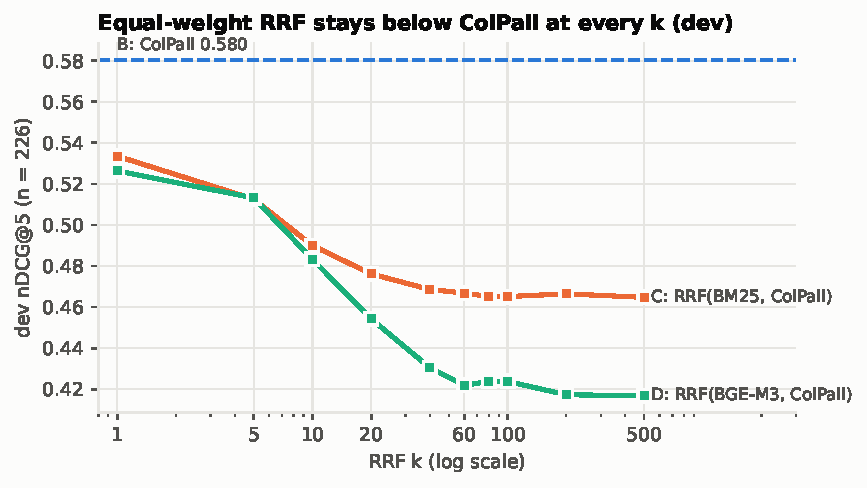
\includegraphics[width=0.62\linewidth]{fig2_dev_k_sweep.pdf}\\[4pt]
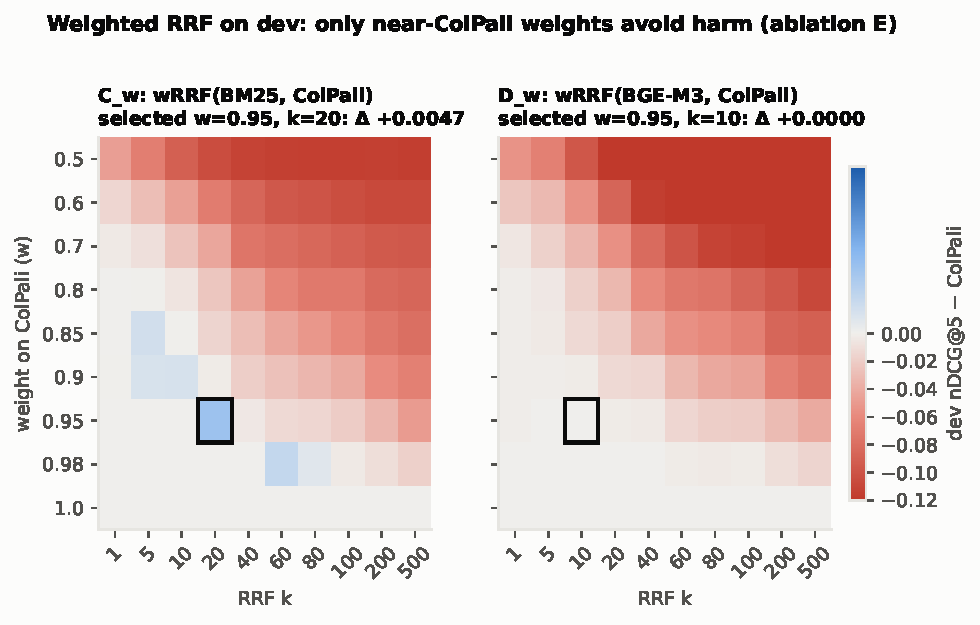
\includegraphics[width=\linewidth]{fig3_dev_weighted_rrf.pdf}
\caption{\Mea{} Dev only. Top: nDCG@5 vs RRF $k$ for C and D, with ColPali as reference. Bottom: $\Delta$nDCG@5 vs ColPali over the weighted-RRF grid ($w \times k$) for C$_w$ and D$_w$.}\label{fig:dev}
\end{figure}

\FloatBarrier
\subsection{Single test run}
\begin{table}[!htbp]\centering\footnotesize\setlength{\tabcolsep}{4pt}
\begin{adjustbox}{max width=\linewidth}
\begin{tabular}{llllllll}
\toprule
System & Role & nDCG@5 [95\% CI] & R@5 & R@10 & MRR@10 & $\Delta$ vs B [95\% CI] & $p_\mathrm{Holm}$ \\
\midrule
A & text baseline & 0.382 [0.323, 0.441] & 0.444 & 0.498 & 0.369 & $-$0.188 [$-$0.237, $-$0.142] & $<$0.001 \\
BGE-M3 & D's text part & 0.262 [0.209, 0.317] & 0.307 & 0.418 & 0.262 & $-$0.308 [$-$0.364, $-$0.252] & $<$0.001 \\
B & reproduced baseline & 0.570 [0.510, 0.627] & 0.653 & 0.680 & 0.546 & -- & -- \\
C & proposed & 0.516 [0.457, 0.574] & 0.618 & 0.667 & 0.489 & $-$0.054 [$-$0.076, $-$0.032] & $<$0.001 \\
D & control & 0.519 [0.460, 0.578] & 0.609 & 0.667 & 0.496 & $-$0.051 [$-$0.072, $-$0.030] & $<$0.001 \\
C$_w$ & ablation E & 0.571 [0.511, 0.629] & 0.653 & 0.680 & 0.547 & +0.001 [$-$0.002, +0.005] & 1.000 \\
D$_w$ & ablation E & 0.570 [0.510, 0.627] & 0.653 & 0.680 & 0.546 & +0.000 [+0.000, +0.000] & 1.000 \\
\bottomrule
\end{tabular}
\end{adjustbox}
\par\smallskip{\footnotesize Test split, 225 queries, run once with settings frozen on dev. CI: percentile bootstrap over queries (10{,}000 resamples). $p$: two-sided paired sign-flip permutation test (10{,}000), Holm-corrected over the six comparisons with B.}

\caption{\Mea{} Test split, all frozen systems (\file{results/test\_evaluation/metrics.json}).}\label{tab:test}
\end{table}

\begin{figure}[!htbp]\centering
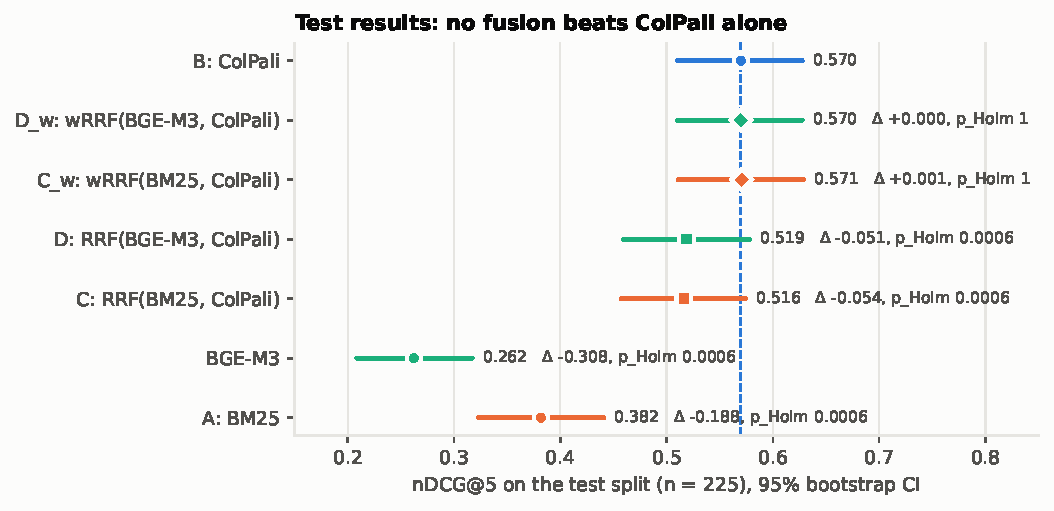
\includegraphics[width=0.85\linewidth]{fig1_test_ndcg5.pdf}
\caption{\Mea{} Test nDCG@5 with 95\% bootstrap CIs. The annotations give $\Delta$ vs ColPali and the Holm-corrected $p$.}\label{fig:test}
\end{figure}

\noindent\textbf{P1 (C $>$ B): rejected.} \Mea{} C reaches \testC{} vs B \testB{}: $\Delta$ = \deltaC{} (95\% CI \deltaCCI{}), $p_\text{Holm}$ \pHolmC{}. Per query (better/same/worse): \wtlC{}. Fusion with BM25 makes retrieval significantly worse, confirming the dev finding on unseen queries.

\noindent\textbf{P3 (C $>$ D): not supported.} \Mea{} D reaches \testD{} ($\Delta$ vs B \deltaD{}). C$-$D = \deltaCvsD{} (CI \deltaCvsDCI{}, $p$ = \pCvsD{}).
\Int{} The harm is not specific to the lexical signal. It is what happens when ColPali is ensembled with equal weight with a much weaker retriever of either kind.

\noindent\textbf{Ablation E.} \Mea{} The dev-selected weighted fusion C$_w$ is \testCw{} ($\Delta$ \deltaCw{}, CI \deltaCwCI{}, $p$ = \pCw{}). It changes the nDCG@5 of only \cwChanged{} test queries (better/same/worse: \wtlCw{}). D$_w$ is identical to B in the top 5 for every query.
\Int{} The \devCwGainPts{}-point dev gain was selection noise from a 90-configuration search. This is the bias we anticipated when pre-registering E.

\noindent\textbf{Post-hoc, without duplicated query texts} ($n$ = \nNoDup{}). \Mea{} Same picture: B \noDupB{}, C $\Delta$ \noDupDeltaC{}, C$_w$ $\Delta$ \noDupDeltaCw{}.

\FloatBarrier
\subsection{By query type (P2)}
\begin{table}[!htbp]\centering\footnotesize
\begin{adjustbox}{max width=\linewidth}
\begin{tabular}{llll}
\toprule
System & exact ($n$=93) & general ($n$=115) & visual ($n$=17) \\
\midrule
A & 0.617 ($-$0.217, $p<0.001$) & 0.231 ($-$0.160, $p<0.001$) & 0.118 ($-$0.221, $p=0.061$) \\
BGE-M3 & 0.458 ($-$0.376, $p<0.001$) & 0.130 ($-$0.261, $p<0.001$) & 0.088 ($-$0.251, $p=0.058$) \\
B & 0.833 & 0.391 & 0.339 \\
C & 0.774 ($-$0.059, $p<0.001$) & 0.345 ($-$0.046, $p=0.006$) & 0.265 ($-$0.074, $p=0.128$) \\
D & 0.771 ($-$0.063, $p<0.001$) & 0.343 ($-$0.048, $p=0.002$) & 0.331 ($-$0.008, $p=1.000$) \\
C$_w$ & 0.837 (+0.004, $p=1.000$) & 0.390 ($-$0.001, $p=0.743$) & 0.335 ($-$0.004, $p=1.000$) \\
D$_w$ & 0.833 (+0.000, $p=1.000$) & 0.391 (+0.000, $p=1.000$) & 0.339 (+0.000, $p=1.000$) \\
\bottomrule
\end{tabular}
\end{adjustbox}
\par\smallskip{\footnotesize Test nDCG@5 by frozen query tag; in brackets $\Delta$ vs B and the uncorrected permutation $p$ (exploratory).}

\caption{\Mea{} Test nDCG@5 by frozen query tag. Exploratory, uncorrected.}\label{tab:type}
\end{table}

\begin{figure}[!htbp]\centering
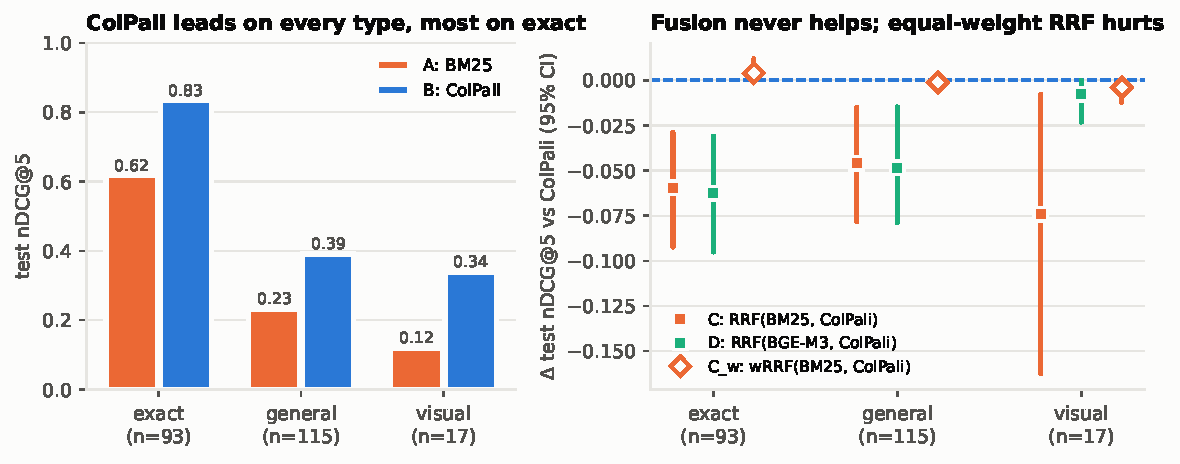
\includegraphics[width=0.95\linewidth]{fig4_test_by_type.pdf}
\caption{\Mea{} Test nDCG@5 by query type (left) and $\Delta$ of each fusion vs ColPali (right).}\label{fig:type}
\end{figure}

\noindent\textbf{P2: not supported.} \Mea{} There is no gain on any query type (Table~\ref{tab:type}, Figure~\ref{fig:type}).
The premise is also contradicted. ColPali is strongest on exact-match queries (\typeexactB{}), well ahead of BM25 (\typeexactA{}), and C loses there too (\typeexactC{}). BM25 is nearly useless on visual queries (\typevisualA{}); C loses most there, but $n$ = \nvisual{} and the difference is not significant.

\FloatBarrier
\subsection{Resources}
\begin{table}[!htbp]\centering\footnotesize
\begin{adjustbox}{max width=\linewidth}
\begin{tabular}{lrrrrr}
\toprule
System & Index time (s) & Index size (MB) & Latency seq.\ (ms) & Latency par.\ (ms) & Fusion (ms) \\
\midrule
A & 0.35 & 0.63 & 0.12 & 0.12 & 0.00 \\
BGE-M3 & 21.10 & 1.95 & 29.04 & 29.04 & 0.00 \\
B & 111.70 & 125.85 & 51.30 & 51.30 & 0.00 \\
C & 112.04 & 126.48 & 51.55 & 51.43 & 0.13 \\
D & 132.79 & 127.81 & 80.47 & 51.43 & 0.13 \\
C$_w$ & 112.04 & 126.48 & 51.56 & 51.44 & 0.14 \\
D$_w$ & 132.79 & 127.81 & 80.47 & 51.43 & 0.13 \\
\bottomrule
\end{tabular}
\end{adjustbox}
\par\smallskip{\footnotesize Medians over single queries. Components were measured on different devices: ColPali on an NVIDIA L4 (bf16, peak GPU memory 15.8~GiB), BGE-M3 on Apple M5 MPS (fp16), BM25 and fusion on the M5 CPU. Sequential = sum of components + fusion; parallel = slowest component + fusion.}

\caption{\Mea{} Resource cost per system (\file{results/test\_evaluation/metrics.json}, field \texttt{resources}).}\label{tab:res}
\end{table}

\noindent\Mea{} Fusion itself costs about \fusionOverhead{}\,ms per query. C adds BM25's 0.35\,s indexing and 0.6\,MB index to ColPali's \idxB{}\,s and \sizeB{}\,MB. If the retrievers run in parallel, query latency is set by ColPali (about \latB{}\,ms on the L4).
\Int{} Fusion is therefore essentially free in this setting. The obstacle is quality, not cost. The cross-device latencies are not directly comparable (Section~\ref{sec:limits}).
\Mea{} ColPali's peak GPU memory was \peakGPU{}\,GiB, far above the size of its bf16 weights.
\Hyp{} The language-model head may compute logits over the full vocabulary during encoding. This was not investigated.

\FloatBarrier
\subsection{Failure analysis}
\label{sec:failure}
All analyses on the test split are post-hoc and descriptive (\file{scripts/failure\_analysis.py}, \file{results/failure\_analysis/}).

\begin{table}[!htbp]\centering\small
\begin{adjustbox}{max width=\linewidth}
\begin{tabular}{lrrrrrr}
\toprule
Tag ($n$) & B hit & A hit & A only & B only & neither & A or B \\
\midrule
all (225) & 147 & 100 & 3 & 50 & 75 & 150 \\
exact (93) & 84 & 62 & 0 & 22 & 9 & 84 \\
general (115) & 56 & 36 & 3 & 23 & 56 & 59 \\
visual (17) & 7 & 2 & 0 & 5 & 10 & 7 \\
\bottomrule
\end{tabular}
\end{adjustbox}
\par\smallskip{\footnotesize Test split; hit = gold page in the top 5. ``A only'' bounds what any fusion of A and B could gain at cut-off 5.}

\caption{\Mea{} Who finds the gold page in the top 5, test split.}\label{tab:headroom}
\end{table}

\paragraph{Headroom.} \Mea{} ColPali has the gold page in its top 5 for \hitB{} test queries and BM25 for \hitA{}. BM25 succeeds where ColPali fails on only \headallAnotB{} queries, none of them exact-match. The reverse happens on \headallBnotA{} (Table~\ref{tab:headroom}, Figure~\ref{fig:fail}, top).
Even an oracle that always picked the right system would reach \oracle{} hits instead of \hitB{}.
\Int{} BM25's successes are almost a subset of ColPali's, so fusion has almost nothing to gain and a lot to lose. This explains P1 and P3.

\paragraph{How C loses.} \Mea{} In \cLossBMmissed{} of C's \cLosses{} losses, BM25 had missed the gold page. Its wrong top pages were pulled above ColPali's correct one, typically moving the gold page from rank~1 to rank~2--5.

\paragraph{Mechanism: lexical overlap after OCR.} \Mea{} Define the overlap as the share of a query's BM25 tokens that occur in the gold page's OCR tokens.
\begin{itemize}
  \item Mean overlap is \ovAhit{} when BM25 hits and \ovAmiss{} when it misses.
  \item With zero overlap (\ovZeroN{} queries), BM25 hits \ovZeroA{}\% and ColPali still \ovZeroB{}\%.
  \item With full overlap (\ovOneN{} queries), BM25 hits \ovOneA{}\% and ColPali \ovOneB{}\% (Figure~\ref{fig:fail}, bottom).
\end{itemize}
\Int{} BM25 only works when the query's words survive OCR and tokenisation. ColPali reads the page image and still matches when the OCR text lacks the words.

\begin{figure}[!htbp]\centering
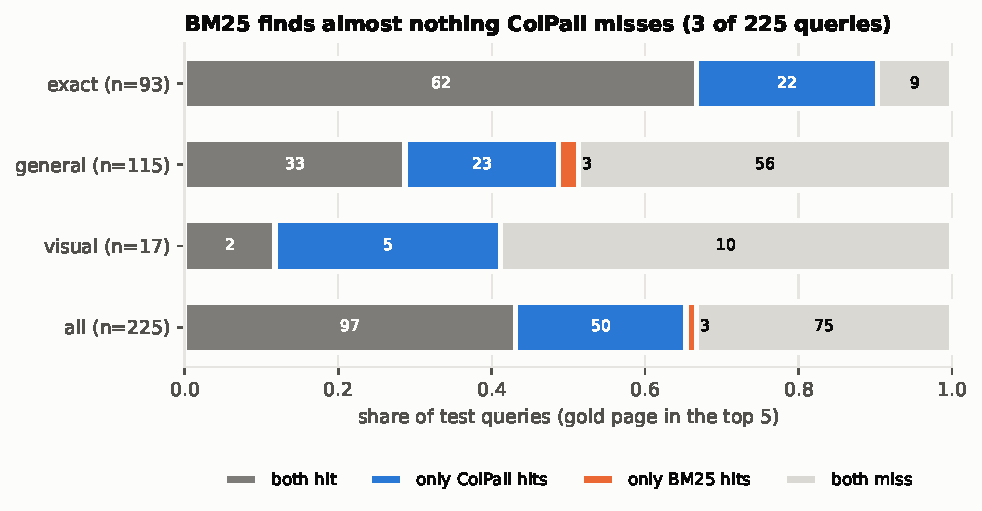
\includegraphics[width=0.8\linewidth]{fig5_headroom.pdf}\\[4pt]
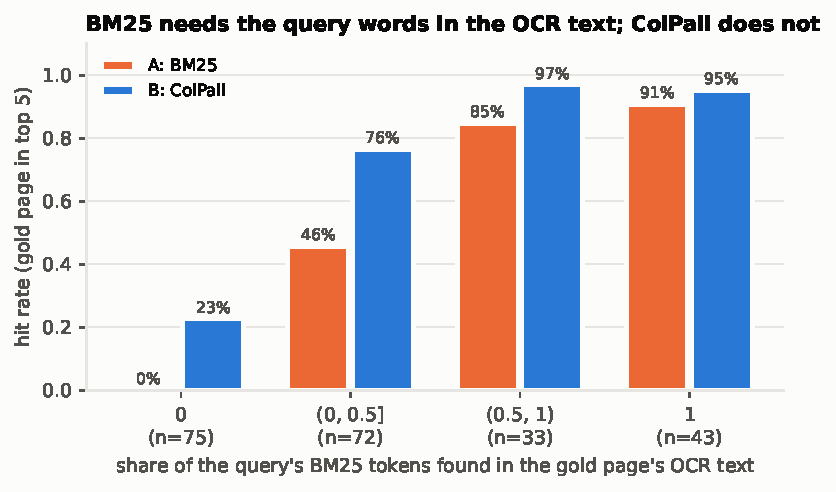
\includegraphics[width=0.8\linewidth]{fig6_overlap.pdf}
\caption{\Mea{} Top: per query type, which system has the gold page in its top 5. Bottom: top-5 hit rate vs query--OCR lexical overlap.}\label{fig:fail}
\end{figure}

\paragraph{Unfavourable examples (C worse than ColPali).} \Mea{} Ranks of the gold page; all examples are in \file{results/failure\_analysis/examples.md}.
\begin{itemize}
  \item \emph{``What is No.~2-26 of subheading H?''} (exact): ColPali~1, BM25~342, C~3. ``No'' is a stopword and ``2-26'' is not alphanumeric, so the anchor never reaches BM25.
  \item \emph{``What is the VO.~NO.?''} (exact): OCR reads ``YO.~NO.''; ColPali~1, BM25~137, C~3.
  \item \emph{``What is the cost of postage (see the postal stamp at top left)?''} (visual): the gold page has \emph{empty} OCR text; ColPali~3, BM25~252, C~7. C$_w$ also moves it from 3 to 4.
  \item \emph{``What Tobacco brand of GPI is shown in the picture?''} (visual): ColPali~1, BM25~31, C~3.
\end{itemize}

\paragraph{Favourable examples (C better than ColPali).} \Mea{} All \cWins{} are listed in the repository. Most are small corrections from rank~2 to rank~1 where BM25 is also right, e.g.\ \emph{``Who is from Indiana?''} and \emph{``When is the remittance due?''}. Two are larger rescues:
\begin{itemize}
  \item \emph{``What is the name of the laboratory?''}: ColPali~14, BM25~3, C~4.
  \item \emph{``How many bullet points are there?''}: ColPali~136, BM25~2, C~4.
\end{itemize}
\Int{} The second rescue is likely lucky: the query's words are generic, not a lexical anchor.

\paragraph{Summary of the verdicts.} P1 rejected (significant harm); P2 not supported (no gain anywhere, and the premise is reversed); P3 not supported (C $\approx$ D). The dev-tuned weighting ties with ColPali.

% =====================================================================================================
\section{Limitations, conclusions and open questions}
\label{sec:limits}

\paragraph{Limitations.}
\begin{itemize}
  \item \textbf{One task, one OCR, one checkpoint.} All conclusions are about ViDoRe~v1 DocVQA with the benchmark's Tesseract text and ColPali~v1.3. \Int{} DocVQA's training split is part of ColPali's training data, which favours ColPali against zero-shot text baselines on this task~\cite[§4.2]{colpali}.
  \item \textbf{Small test set.} 225 queries; 17 visual queries. Per-type results are exploratory, and the confidence intervals are wide (about $\pm$0.06 nDCG@5 per system).
  \item \textbf{Rank fusion only.} We did not try score-level convex combination with normalisation, which Bruch et al.\ found better than RRF~\cite{bruch}. \Int{} The headroom analysis bounds any fusion of these two rankings at cut-off 5, at \headallAnotB{} extra hits, so a better fusion function cannot change the conclusion much.
  \item \textbf{Official BM25 preprocessing.} It drops stopwords such as ``no'' and non-alphanumeric tokens such as ``2-26''. We kept it for comparability with the paper. A code-preserving tokenizer is a separate, untested change.
  \item \textbf{Coarse query tags.} The rule-based tags miss rare lowercase terms and count generic capitalised labels as anchors.
  \item \textbf{Mixed hardware.} Resource numbers were measured on different devices (L4 GPU, M5 MPS, M5 CPU), so cross-system latency sums are indicative only.
  \item \textbf{Reproduction gap not isolated.} The \gapCardPts{}-point gap was not traced to a cause. We reproduced v1.3, not the paper's v1.0.
  \item \textbf{Literature search.} The search was small and was done with AI assistance; the research gap was narrowed after the experiments (Section~\ref{sec:lit}).
\end{itemize}

\paragraph{Conclusions.}
\begin{itemize}
  \item \Mea{} ColPali's DocVQA result is reproducible with the authors' code and checkpoint (\fullB{} vs \pubCard{}).
  \item \Mea{} Adding BM25 through RRF significantly \emph{hurts} it (\deltaC{} nDCG@5 on test). A dense-text control hurts equally. The best dev-tuned weighting only ties.
  \item \Int{} On this task ColPali already reads the lexical anchors that BM25 depends on, and reads them better than Tesseract OCR does. Equal-weight rank fusion with a much weaker second ranking therefore mostly imports that ranking's errors. This is consistent with the conditions under which fusion is reported to fail in text IR~\cite{bruch}, and with the cases where text + visual fusion did help having clean text and comparably strong inputs~\cite{irpapers}.
\end{itemize}

\paragraph{Open questions.}
\begin{itemize}
  \item \Hyp{} A lexical signal should start to help when the page text improves (layout-aware or LLM-based OCR, a tokenizer that keeps codes), or on text-dense corpora where text retrieval is close to visual retrieval. Testing this needs a task where the headroom (``A only'' in Table~\ref{tab:headroom}) is large.
  \item \Hyp{} On ViDoRe~V2, which reduces query--page lexical overlap by design~\cite{vidorev2}, fusion should help even less.
  \item Open: why does ColPali v1.3 use about \peakGPU{}\,GiB of GPU memory to encode pages?
\end{itemize}

% =====================================================================================================
\appendix
\section{Reproducibility}
\label{app:repro}
\begin{itemize}
  \item \textbf{Repository and version:} \repo{}. The reported version is tag \texttt{v1.0-submission} \todo{tag}.
  \item \textbf{Dependencies:} pinned in \file{requirements.txt}; the Colab \texttt{pip freeze} is in\\\file{results/colpali\_v1.3\_docvqa/}.
  \item \textbf{Model and data revisions:} pinned in \file{configs/*.yaml}.
  \item \textbf{Every run, including failed ones:} UTC time, machine, commit and log path in \file{docs/run\_registry.md}. The reasoning behind decisions is in \file{docs/experiment\_log.md}; deviations are in \file{docs/deviations.md}.
\end{itemize}

\noindent\textbf{GPU (once).} ColPali scores:
\begin{Verbatim}[fontsize=\footnotesize,breaklines=true]
python scripts/run_colpali.py --config configs/colpali_v1.3_docvqa.yaml
\end{Verbatim}
On Colab, use \file{notebooks/colpali\_docvqa\_colab.ipynb} with an L4 runtime.

\noindent\textbf{CPU, seconds, no GPU or model download needed.} These read only committed files:
\begin{Verbatim}[fontsize=\footnotesize,breaklines=true]
python scripts/run_bm25.py --config configs/bm25_docvqa.yaml
python scripts/run_bge_m3.py --config configs/bge_m3_docvqa.yaml      # ~1 min, MPS/GPU
python scripts/make_split.py --seed 0 --dev-fraction 0.5
python scripts/run_fusion_dev.py --config configs/fusion_docvqa.yaml
python scripts/run_weighted_fusion_dev.py --config configs/fusion_weighted_docvqa.yaml
python scripts/run_test_evaluation.py --config configs/test_evaluation.yaml
python scripts/failure_analysis.py
python scripts/make_figures.py
python scripts/make_report_tables.py && (cd report && tectonic main.tex)
python -m pytest -q tests                                             # fast tests
\end{Verbatim}

\section{AI-use disclosure}
\label{app:ai}
AI assistance was used and is permitted by the assignment. The detailed, dated record is \file{docs/ai\_usage.md}.
\begin{itemize}
  \item \textbf{Claude (claude.ai chat):} topic scoping and the first draft of the research plan.
  \item \textbf{Claude Code (Claude Opus~5.5)} did the following:
  \begin{itemize}
    \item wrote most of the code and tests;
    \item drove the Colab notebook through a browser (the author signed in);
    \item ran the local experiments;
    \item extracted literature details from the papers;
    \item drafted the documentation, the figures and this report.
  \end{itemize}
\end{itemize}
The author chose the topic, task, checkpoint, control model and every pre-registration step; approved each run; and is responsible for reading the sources, checking citations and every claim, and defending the conclusions. \todo{author: describe what you verified yourself, e.g.\ papers read, code reviewed, examples checked against page images}

% =====================================================================================================
\begin{thebibliography}{99}\small
\bibitem{colpali} M.~Faysse, H.~Sibille, T.~Wu, B.~Omrani, G.~Viaud, C.~Hudelot, P.~Colombo. ColPali: Efficient Document Retrieval with Vision Language Models. arXiv:2407.01449v6, 2025. \todo{verify venue (ICLR 2025?)}
\bibitem{colbert} O.~Khattab, M.~Zaharia. ColBERT: Efficient and Effective Passage Search via Contextualized Late Interaction over BERT. SIGIR 2020. doi:10.1145/3397271.3401075.
\bibitem{dse} X.~Ma, S.-C.~Lin, M.~Li, W.~Chen, J.~Lin. Unifying Multimodal Retrieval via Document Screenshot Embedding. EMNLP 2024 (arXiv:2406.11251v2).
\bibitem{vidorev2} Q.~Macé, A.~Loison, M.~Faysse. ViDoRe Benchmark V2: Raising the Bar for Visual Retrieval. arXiv:2505.17166v2, 2025.
\bibitem{cormack} G.~V.~Cormack, C.~L.~A.~Clarke, S.~Büttcher. Reciprocal Rank Fusion outperforms Condorcet and individual Rank Learning Methods. SIGIR 2009. doi:10.1145/1571941.1572114.
\bibitem{bruch} S.~Bruch, S.~Gai, A.~Ingber. An Analysis of Fusion Functions for Hybrid Retrieval. arXiv:2210.11934v2, 2023 (related DOI 10.1145/3596512). \todo{verify venue}
\bibitem{irpapers} C.~Shorten, A.~Skaburskas, D.~M.~Jones, C.~Pierse, R.~Esposito, J.~Trengrove, E.~Dilocker, B.~van~Luijt. irpapers: A Visual Document Benchmark for Scientific Retrieval and Question Answering. arXiv:2602.17687v1, 2026.
\bibitem{slides} P.~S.~Giouroukis, D.~Dimitriadis, D.~Papadopoulos, Z.~Shao, G.~Tsoumakas. What's the Best Way to Retrieve Slides? A Comparative Study of Multimodal, Caption-Based, and Hybrid Retrieval Techniques. arXiv:2509.15211v1, 2025. \todo{verify venue}
\bibitem{lostocr} A.~Most, J.~Winjum, A.~Biswas, S.~Jones, N.~R.~Ranasinghe, D.~O'Malley, M.~Bhattarai. Lost in OCR Translation? Vision-Based Approaches to Robust Document Retrieval. ACM DocEng 2025 (arXiv:2505.05666v1).
\bibitem{beir} N.~Thakur, N.~Reimers, A.~Rücklé, A.~Srivastava, I.~Gurevych. BEIR: A Heterogenous Benchmark for Zero-shot Evaluation of Information Retrieval Models. NeurIPS 2021 Datasets and Benchmarks.
\bibitem{visrag} S.~Yu, C.~Tang, B.~Xu, J.~Cui, J.~Ran, Y.~Yan, Z.~Liu, S.~Wang, X.~Han, Z.~Liu, M.~Sun. VisRAG: Vision-based Retrieval-augmented Generation on Multi-modality Documents. arXiv:2410.10594v2, 2025.
\end{thebibliography}

\end{document}
